\documentclass[11pt]{article}
\usepackage[T1]{fontenc}
\usepackage{lmodern,amsmath,booktabs,graphicx}
\usepackage[margin=1in]{geometry}
\usepackage[colorlinks=true,linkcolor=blue,citecolor=blue,urlcolor=blue]{hyperref}
\hypersetup{pdfauthor={Qianghao Wu},pdftitle={A pre-registered forward test of 86 ZTF periodic-quasar candidates finds no predictive periodicity}}
\title{A pre-registered forward test of 86 ZTF periodic-quasar candidates finds no predictive periodicity}
\author{Qianghao Wu}
\date{November 25, 2026}
\emergencystretch=3em
\begin{document}
\maketitle
\begin{abstract}
Chen et al.\ (2024) searched the ZTF DR11 light curves of 143,700 quasars and reported 86 candidates with significant sinusoidal variation against a single power-law red-noise model. Three of them still met the selection criteria in longer archival light curves. A stable sinusoid must continue after the data that found it. We froze the sinusoid of each candidate on the DR11 epochs and scored its prediction of the next 3.6 years of public ZTF r-band data (median 1.42 cycles). We wrote down the test, the controls and the decision rule before we computed any score. Each score was calibrated against damped-random-walk mocks that look at least as periodic as the candidate in the DR11 window. 7 of 86 candidates beat their mocks at $p<0.05$, where chance gives 4.3 (binomial $p=0.139$). 29 of 273 magnitude- and redshift-matched quasars that were not selected for periodicity do the same (10.6\%; Fisher $p=0.81$). None of the three named candidates is confirmed: their $p$-values are 0.26, 0.81 and 0.40. So we find no evidence that the candidate population continues as strict sinusoids. If all 86 were strict sinusoids at their fitted amplitude, simulations predict 65 passes. At 95\% confidence, at most 14\% of the candidates are strict sinusoids with the simulated power, or at most 36\% with the lower power that we measured by injection into real quasar light curves (post hoc). The test does not exclude quasi-periodic signals, which Chen et al.\ already proposed as an explanation.

This work has not yet been reviewed by experts. The computations, the code and the text were produced by AI models (from Anthropic and OpenAI), working under the author's direction.
\end{abstract}
\medskip
\noindent\textit{Keywords:} quasars, periodic variability, supermassive black hole binaries, red noise, Zwicky Transient Facility, pre-registration

\section{Introduction}
A close binary of supermassive black holes can make the optical light of a quasar vary with a period of months to years. Many searches look for such periods in survey light curves. Normal quasar variability is red noise: it has more power on long time scales. A red-noise light curve that covers only a few cycles can look periodic. Vaughan et al.\ showed that this effect can explain claimed quasar periodicities~\cite{vaughan2016}. A sinusoid that red noise makes by chance does not continue. So new data after the search are a direct test.

Several candidate lists have been tested with later data. Liu et al.\ found 3 periodic candidates among 670 quasars in Pan-STARRS1 field MD09. None stayed periodic over an extended baseline of 7 to 14 years~\cite{liu2016}. Graham et al.\ reported 111 candidates from the Catalina Real-Time Transient Survey (CRTS)~\cite{graham2015}. Foustoul et al.\ added ZTF data to 58 earlier CRTS candidates and attributed their modulation to red noise~\cite{foustoul2025}. Charisi et al.\ reported candidates from the Palomar Transient Factory (PTF)~\cite{charisi2016}. Robnik et al.\ reassessed them with null-signal templates~\cite{robnik2024}. El-Badry, Hogg and Rix took 181 Gaia DR3 candidates. In all 116 cases with ZTF data, the Gaia periodic model did not predict the later variability~\cite{elbadry2025}. Fatovi\'c et al.\ tested period diagnostics on Stripe 82 candidates~\cite{fatovic2026}. We found no test of the ZTF list of Chen et al.\ with data after its search window (Section~\ref{sec:novelty}).

Chen et al.\ searched the ZTF DR11 r-band light curves of 143,700 SDSS and V\'eron-Cetty \& V\'eron quasars~\cite{chen2024}. They write: ``we finally identify 106 (DRW) and 86 (SPL) candidates with the most significant periodic variations out of 143,700 quasars''. They adopt the 86 candidates of the single power-law (SPL) red-noise model as the final sample. In longer light curves from CRTS, PTF, Pan-STARRS1 and ATLAS, ``only three candidates (with 6-8 cycles of periods) meet the selection criteria''. These are SDSS J083111, SDSS J155304 and SDSS J135830. The authors conclude that ``instead of being strictly periodic, the variability must be quasi-periodic or caused by stochastic red-noise'', and that more data are necessary ``to confirm their periodicity and rule out false positives due to red-noise''.

So Chen et al.\ do not claim that all 86 candidates are strict sinusoids. Our result is an independent out-of-sample check of their own conclusion. It is also a new test of the three named candidates. The ZTF public archive now has 3.6 years of data after the DR11 window. This is about 1.4 cycles of the candidates' periods.

\begin{quote}
\textbf{The sinusoids fitted to the ZTF DR11 data of the 86 SPL candidates do not predict the next 3.6 years of ZTF data better than red noise does, and not better than the same procedure does for unselected quasars. None of the three named candidates is confirmed.}
\end{quote}

\section{Data}
\paragraph{Candidates.} The full candidate tables of Chen et al.\ are on the journal site only, which we could not reach. The arXiv source of the paper labels all 86 SPL candidates in its Appendix C figures. We took the names from these figures. 85 are SDSS names, which give J2000 positions. The last, \texttt{2QZJ131914+0027}, is a truncated 2QZ name. Exactly one 2QZ catalogue entry fits the box that the name allows: 2QZ J131914.8+002709~\cite{croom2004}. Redshifts and PSF $r$ magnitudes come from the SDSS DR14 quasar catalogue (DR14Q)~\cite{paris2018} and, for the 2QZ object, from the 2QZ catalogue. The arXiv text gives the GLS period of 5 candidates (Table 1 excerpt). We use these 5 values as a check of our period fits.

\paragraph{Placebo.} For each candidate we drew 4 DR14Q quasars with $|\Delta r|<0.3$ mag, $|\Delta z|<0.3$, $r\le 20$, declination $>-28^\circ$ and no candidate within 10 arcsec. The draw is without replacement and uses a fixed seed. This gives 344 placebo quasars. They are matched in magnitude and redshift only. They are not selected for periodicity.

\paragraph{Light curves.} We downloaded the ZTF r-band epochs~\cite{bellm2019,masci2019} of all 430 objects from the IRSA light-curve service on 2026-11-24. We used all ZTF object IDs within 3 arcsec, the radius of Chen et al. We kept epochs with \texttt{catflags} $=0$. The last epoch is MJD 60969.55 (2025-10-21).

\section{Method}
We committed the protocol to a git repository on 2026-11-24 at 22:53 (+01:00), before we computed a test-window score for any real light curve. The released folder contains the protocol (\texttt{PROTOCOL.md}). Before the commit we ran the training-window steps and the mocks for 5 candidates in a mode that does not score the test window. We also ran synthetic known-answer checks.

\paragraph{Windows.} The training window is the DR11 public selection of the ZTF release notes~\cite{dr11notes}: \texttt{programid} 1 epochs from MJD 58194.0 to 59647.0 (2022-03-09), and \texttt{programid} 2 and 3 epochs to MJD 59159.0. The test window is MJD 59647.0 to 60970.0. Private-survey epochs between MJD 59159 and 59647 are in neither window.

\paragraph{Processing.} We follow the recipe of Chen et al.\ in each window separately. A 15th-order polynomial is fitted, and points more than 3 standard deviations from it are removed. The epochs are then averaged in 20-day bins. An object needs at least 40 training bins (the cut of Chen et al.) and 10 test bins.

\paragraph{Frozen sinusoid.} We compute an unweighted generalised Lomb--Scargle periodogram~\cite{zechmeister2009} of the training bins for periods from 50 d to the training span. At the highest peak we fit $y=c+a\cos(2\pi t/P)+b\sin(2\pi t/P)$. The signal-to-noise $\xi=(a^2+b^2)/(2\,\mathrm{var}(\text{residuals}))$ is the statistic of Chen et al. The template $s(t)=a\cos(2\pi t/P)+b\sin(2\pi t/P)$ is then frozen.

\paragraph{Score.} The forward score $k$ is the least-squares slope of the test-window bins on $s(t)$, with a free offset. If the sinusoid continues with the same amplitude and phase, $k=1$. If it has no predictive skill, $k=0$ on average. The free offset absorbs drifts of the mean level.

\paragraph{Null.} The primary null is a damped random walk (DRW)~\cite{kelly2009}. We fit its two parameters by maximum likelihood to the training bins. Mocks are drawn at the training and test bin times, with the bin errors added. Each mock goes through the same steps: its own periodogram, its own frozen sinusoid and its own $k$. The candidates were selected because they look periodic. So a mock enters the null only if it also looks periodic in training: $\xi_\text{mock}\ge\min(\xi_\text{obs},4)$ and a period within 20\% of the candidate's period. We drew mocks in batches of 20,000 until 1,000 were accepted, up to 300,000. If fewer than 200 were accepted, the object used the unconditioned null, as the protocol states. This happened for 14 of 86 candidates. The one-sided $p$-value $p_\text{DRW}$ is the fraction of null $k$ at or above the observed $k$. A secondary null uses power-law noise with slope $\beta=3$, made with the method of Timmer and K\"onig~\cite{timmer1995}.

\paragraph{Tests and decision rule.} Let $N_C$ of $n_C$ candidates and $N_P$ of $n_P$ placebo objects have $p_\text{DRW}<0.05$.
T1 is a one-sided binomial test of $N_C$ against the rate 0.05.
T2 is a one-sided Fisher exact test of the candidate fraction against the placebo fraction. T2 does not depend on a correct null model, because the placebo goes through the same pipeline.
The protocol says ``Supported'' if T1 and T2 both give $p<0.01$, ``Not supported'' if T1 gives $p\ge 0.01$, and ``Inconclusive'' otherwise. A named candidate counts as confirmed if $p_\text{DRW}<0.05/3$.

\paragraph{Power and injection.} For each candidate we simulated 2,000 light curves as the frozen sinusoid plus a DRW fitted to the training residuals. The power is the fraction of these with $k$ above the 95th percentile of the null. In a second control we added each candidate's frozen sinusoid to the raw epochs of its first placebo quasar and ran the full pipeline.

\paragraph{Changes after the protocol.} We fixed the end of the test window at MJD 60970.0, after the last epoch, so that a rerun after a new ZTF release gives the same numbers. Five placebo objects have no r-band data; we added a numeric conversion so that they are excluded instead of stopping the run. A post hoc block (injection-based limits and a Bonferroni count) was added and is labelled as such. No test, threshold or sample changed.

\section{Results}
\paragraph{Population.} All 86 candidates and 273 of 344 placebo quasars have enough bins. 71 placebo objects were excluded for sampling, 5 of them with no r-band data. The candidates have training periods from 601 to 1030 d (median 872 d). Our refit periods for the 5 published values are 783, 740, 739, 630 and 698 d, against 788.8, 736.2, 736.2, 626.6 and 688.6 d. The median test window has 40.5 bins and 1.42 cycles.

\begin{center}
\begin{tabular}{lrrl}
\toprule
Test & Value & $p$ & Threshold \\
\midrule
T1: candidates with $p_\text{DRW}<0.05$ & 7 of 86 (8.1\%); chance 4.3 & 0.139 & 0.01 \\
T2: candidates against placebo & 7/86 against 29/273 (10.6\%) & 0.81 & 0.01 \\
\midrule
Decision & \multicolumn{3}{l}{\textbf{Not supported}} \\
\bottomrule
\end{tabular}
\end{center}

The median $k$ is 0.10 for the candidates and 0.02 for the placebo (Mann--Whitney one-sided $p=0.16$). For the injected sinusoids it is 0.37. If all 86 candidates were strict sinusoids at their fitted amplitude, the simulated power (mean 0.76) predicts 65.4 candidates at $p_\text{DRW}<0.05$. We observe 7. Figure~\ref{fig:k} shows the distributions of $k$ and $p_\text{DRW}$.

\begin{figure}[t]
\centering
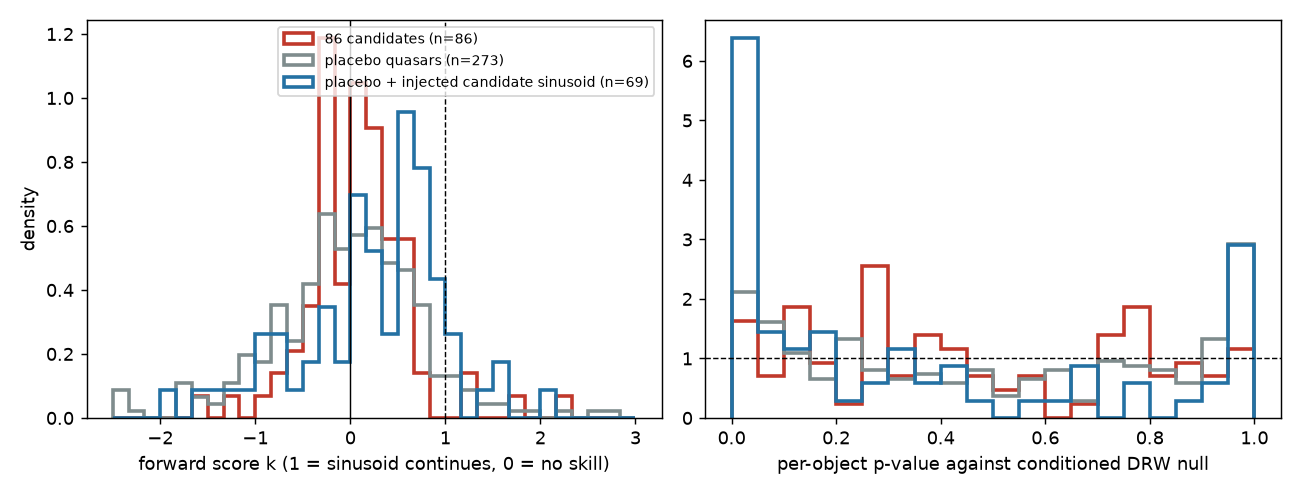
\includegraphics[width=\textwidth]{../data/fig_forward_score.png}
\caption{Left: forward score $k$ for the candidates, the placebo quasars and the placebo quasars with an injected candidate sinusoid. Right: per-object $p_\text{DRW}$. A calibrated null gives a flat histogram (dashed line). The candidates and the placebo look alike. The injected sinusoids give larger $k$ and more small $p$-values.}
\label{fig:k}
\end{figure}

\paragraph{Upper limit.} The protocol defines $f_{95}$ as the smallest fraction $f$ of strict sinusoids for which 7 or fewer passes have probability at most 0.05. With the simulated power, $f_{95}=0.138$. The fitted amplitudes of selected candidates are biased high, so this power is optimistic. Post hoc, with the injection pass rate (0.32) as the power, $f_{95}=0.363$. With the placebo pass rate (0.106) as the chance rate, it is 0.194.

\paragraph{Amplitude and phase.} A sinusoid refitted to the test window at the frozen period has median amplitude 0.46 times the training amplitude. 25.6\% of the candidates have a phase shift within $\pm0.125$ cycle. Chance gives 25\%, and the placebo gives 30.8\%.

\paragraph{Individual candidates.} The smallest candidate $p_\text{DRW}$ is 0.0029 (SDSS J132457.51+325145.9). The Bonferroni threshold for 86 tests is 0.00058. So no candidate passes a correction for multiple tests. The 7 nominal passes are SDSS J102435.39+372637.0, J110837.68+100333.1, J113543.22+592241.8, J120722.30+204340.2, J122805.51+061655.4, J125156.26+194224.3 and J132457.51+325145.9. Their number is consistent with chance. They are the natural targets for further monitoring.

\paragraph{The three named candidates.} None is confirmed (Figure~\ref{fig:named}). SDSS J083111 keeps its phase, but its amplitude falls to 24\% of the training value. SDSS J155304 is almost in anti-phase.

\begin{center}
\begin{tabular}{lrrrrrr}
\toprule
Object & $P$ (d) & $k$ & $p_\text{DRW}$ & Phase shift & Amplitude ratio & Power \\
\midrule
SDSS J083111.23+123107.8 & 885 & 0.24 & 0.257 & $-0.000$ & 0.24 & 0.85 \\
SDSS J155304.40+240255.1 & 886 & $-0.30$ & 0.812 & $+0.45$ & 0.32 & 0.96 \\
SDSS J135830.46$-$012255.7 & 746 & 0.11 & 0.399 & $+0.22$ & 0.29 & 0.90 \\
\bottomrule
\end{tabular}
\end{center}

\begin{figure}[t]
\centering
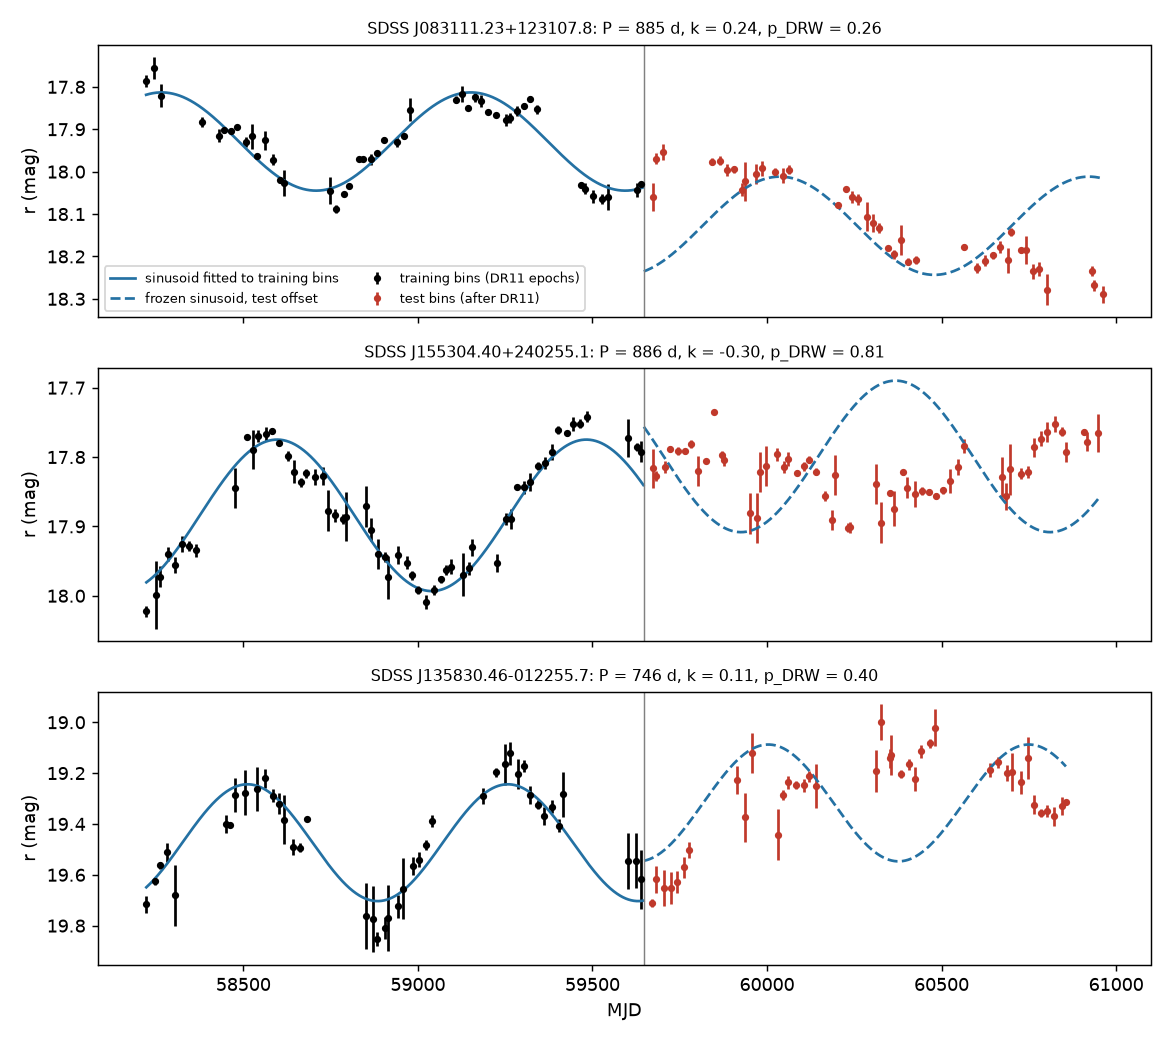
\includegraphics[width=0.9\textwidth]{../data/fig_named.png}
\caption{The three candidates that Chen et al.\ found periodic also in extended data. Black: training bins (DR11 epochs). Red: test bins. Solid line: the sinusoid fitted to the training bins. Dashed line: the same sinusoid, frozen, with the offset of the test bins. The vertical line is the end of the DR11 public epochs (MJD 59647).}
\label{fig:named}
\end{figure}

\section{Controls}
\paragraph{Placebo and null calibration.} 29 of 273 placebo quasars (10.6\%) have $p_\text{DRW}<0.05$. A calibrated null gives 5\%. So the conditioned DRW null is anti-conservative by about a factor of 2, and the exact T1 $p$-value is not reliable. The unconditioned DRW null gives 15 of 273 (5.5\%) for the placebo and 3 of 86 for the candidates. The excess therefore comes with the selection conditioning. We did not find its cause. The conclusion does not rest on T1 alone. The candidate rate (8.1\%) is below the placebo rate. A miscalibrated null makes passes more frequent, not less. T2 is free of the null model.

Only 1 placebo quasar passes $\xi>4$ and more than 1.5 training cycles, the first cut of Chen et al. So the planned comparison with a ``near-miss'' placebo subset was not possible. T2 compares the candidates with unselected quasars.

\paragraph{Injection.} The injected sinusoids give 22 passes in 69 analysed cases (32\%; 17 hosts had too few bins). This shows that the test detects real sinusoids of the candidates' amplitude in real quasar light curves. The power is lower than in the simulations (0.76). One reason is that the host light curve keeps its own red noise. Its median DRW amplitude is 0.117 mag, against a median injected amplitude of 0.115 mag. In the simulations, the noise is the DRW fitted to the residuals of the sinusoid, with median amplitude 0.028 mag. In an independent rerun, the training periodogram recovered the injected period within 10\% in only 46\% of the injections. The median $k$ was 0.67 when the period was recovered and 0.07 when it was not.

\paragraph{Power-law null.} With the $\beta=3$ power-law null, 1 of 86 candidates and 4 of 273 placebo quasars pass. Its mean power is 0.08. We stated in the protocol, before the result, that this null has almost no power here.

\section{How the result was checked}
\paragraph{Reruns.} A rerun from a clean copy of the repository downloaded all public data again and reproduced all 164 numbers of the summary file (relative tolerance $10^{-3}$). On Linux, the Monte Carlo $p$-values of 6 of the 516 objects differ by at most 0.016, because a floating-point difference can change which mocks pass the acceptance threshold. All counts and all numbers in this paper are the same on both platforms. A second clean-copy rerun by a separate verification session gave byte-identical summary and per-object tables and byte-identical light curves. It also rebuilt both sample tables from fresh catalogue downloads, with identical results.

\paragraph{Independent code.} The verification session wrote its own code, with no import of ours. It used a Legendre polynomial clip, the \texttt{astropy} Lomb--Scargle periodogram and its own DRW likelihood. For all 359 analysed objects, the periods agree to a relative $4.5\times10^{-5}$. The scores $k$ agree to a median relative $7\times10^{-6}$. T1, T2 and the Mann--Whitney test from the table agree exactly. Independent conditioned DRW $p$-values for 21 objects agree within Monte Carlo noise. For the named candidates they are 0.260, 0.389 and 0.787, against our 0.257, 0.399 and 0.812. Model-free checks also agree with no signal: 58.1\% of the candidates have $k>0$ (binomial $p=0.080$ against 0.5), a Wilcoxon signed-rank test on $k$ gives $p=0.122$, and a Mann--Whitney test on the test-window correlation of candidates against placebo gives $p=0.172$.

\paragraph{Sensitivity.} Two nominal passes, SDSS J110837.68+100333.1 and SDSS J113543.22+592241.8, have $p_\text{DRW}=0.046$ and 0.044. The independent Monte Carlo gives 0.050 and 0.052. So $N_C$ is between 5 and 7, depending on the random draws. The decision does not change: T1 needs $N_C\ge 11$ for $p<0.01$ ($N_C=10$ gives 0.0107). The 15th-order polynomial fit is poorly conditioned. A different polynomial basis changes the clipped points for 17 of 359 objects and moves $k$ by at most 0.056. The 5 affected candidates have $p_\text{DRW}$ from 0.15 to 1.0, so $N_C$ does not change. Two affected placebo objects are near the threshold, so $N_P$ can change by 1 or 2. This does not change T2.

\section{Limits}
\begin{itemize}
\item The test is for the model of the search: a stable sinusoid. The median test window has 1.42 cycles. A quasi-periodic signal, or a signal whose period or amplitude changes, can fail this test and still be real. Chen et al.\ already proposed such signals.
\item We do not rule out individual candidates. A single candidate with $p_\text{DRW}$ of 0.2 is not excluded. The result is about the population.
\item The 14\% limit assumes that the fitted training amplitude is the true amplitude and that little red noise remains. Both assumptions favour detection. The injection-based 36\% limit uses real quasar noise. It was chosen after the result.
\item Our pipeline follows the recipe of Chen et al.\ but is not identical. We use the current ZTF photometry, which was reprocessed after DR11, \texttt{catflags} $=0$, an unweighted periodogram and DRW fits on binned data. We do not repeat their autocorrelation step or their red-noise model fits. 74\% of our refits have $\xi>4$. Our periods agree with the 5 published values within 1.4\%.
\item We did not test the 106 candidates of the DRW list. Their names are only in the journal tables.
\end{itemize}

\section{Novelty and related work}\label{sec:novelty}
We searched the citations of Chen et al.\ (25 in Semantic Scholar, 47 in OpenAlex), the arXiv, the web, Zenodo and GitHub on 2026-11-24 and 2026-11-25. We found no test of the Chen et al.\ list with ZTF data after DR11. The closest method is the forward test of El-Badry, Hogg and Rix on a different list~\cite{elbadry2025}. Our test adds a pre-registered decision rule, a selection-conditioned red-noise null for each object, a matched placebo of unselected quasars and an injection control. Our result agrees with theirs and with the conclusion of Chen et al.: the strict sinusoids found in a few years of survey data mostly do not continue.

\section{Data and code}
The released folder contains the protocol, the candidate and placebo tables, the per-object results and the scripts. \texttt{checks/rerun.py} downloads the light curves from IRSA, repeats the analysis and compares every number with \texttt{data/expected.json}. \texttt{checks/ci.sh} also compares every per-object value. ZTF data are public; we acknowledge the Zwicky Transient Facility and IRSA. We use SDSS DR14Q and 2QZ catalogue data.

\begin{thebibliography}{20}
\bibitem{chen2024} Y.-J. Chen, S. Zhai, J.-R. Liu et al., Searching for quasar candidates with periodic variations from the Zwicky Transient Facility: results and implications, \emph{MNRAS} 527, 12154--12177 (2024). \href{https://doi.org/10.1093/mnras/stad3981}{doi:10.1093/mnras/stad3981}, \href{https://arxiv.org/abs/2206.11497}{arXiv:2206.11497}. Quotations from the abstract and Sect.~5 of arXiv v2.
\bibitem{vaughan2016} S. Vaughan, P. Uttley, A. G. Markowitz et al., False periodicities in quasar time-domain surveys, \emph{MNRAS} 461, 3145 (2016). \href{https://doi.org/10.1093/mnras/stw1412}{doi:10.1093/mnras/stw1412}.
\bibitem{liu2016} T. Liu, S. Gezari, W. Burgett et al., A systematic search for periodically varying quasars in Pan-STARRS1: an extended baseline test in Medium Deep Survey field MD09, \emph{ApJ} 833, 6 (2016). \href{https://doi.org/10.3847/0004-637X/833/1/6}{doi:10.3847/0004-637X/833/1/6}.
\bibitem{graham2015} M. J. Graham, S. G. Djorgovski, D. Stern et al., A systematic search for close supermassive black hole binaries in the Catalina Real-Time Transient Survey, \emph{MNRAS} 453, 1562 (2015). \href{https://doi.org/10.1093/mnras/stv1726}{doi:10.1093/mnras/stv1726}.
\bibitem{foustoul2025} V. Foustoul, N. A. Webb, R. Mignon-Risse et al., A catalogue of candidate milli-parsec separation massive black hole binaries from long term optical photometric monitoring, \emph{A\&A} 699, A55 (2025). \href{https://doi.org/10.1051/0004-6361/202452818}{doi:10.1051/0004-6361/202452818}.
\bibitem{charisi2016} M. Charisi, I. Bartos, Z. Haiman et al., A population of short-period variable quasars from PTF as supermassive black hole binary candidates, \emph{MNRAS} 463, 2145 (2016). \href{https://doi.org/10.1093/mnras/stw1838}{doi:10.1093/mnras/stw1838}.
\bibitem{robnik2024} J. Robnik, A. E. Bayer, M. Charisi, Z. Haiman et al., Periodicity significance testing with null-signal templates: reassessment of PTF's SMBH binary candidates, \emph{MNRAS} 534, 1609--1620 (2024). \href{https://doi.org/10.1093/mnras/stae2220}{doi:10.1093/mnras/stae2220}.
\bibitem{elbadry2025} K. El-Badry, D. W. Hogg, H.-W. Rix et al., Active galactic nuclei do not exhibit strictly sinusoidal brightness variations, accepted to \emph{PASP}. \href{https://arxiv.org/abs/2509.10601}{arXiv:2509.10601}.
\bibitem{fatovic2026} M. Fatovi\'c et al., Testing period diagnostics on quasar periodic candidates in the era of large surveys, \emph{Serbian Astronomical Journal} 212, 47--66 (2026). \href{https://doi.org/10.2298/SAJ2612047F}{doi:10.2298/SAJ2612047F}.
\bibitem{croom2004} S. M. Croom, R. J. Smith, B. J. Boyle et al., The 2dF QSO Redshift Survey -- XII. The spectroscopic catalogue and luminosity function, \emph{MNRAS} 349, 1397 (2004). \href{https://doi.org/10.1111/j.1365-2966.2004.07619.x}{doi:10.1111/j.1365-2966.2004.07619.x}.
\bibitem{paris2018} I. P\^aris, P. Petitjean, E. Aubourg et al., The Sloan Digital Sky Survey quasar catalog: fourteenth data release, \emph{A\&A} 613, A51 (2018). \href{https://doi.org/10.1051/0004-6361/201732445}{doi:10.1051/0004-6361/201732445}.
\bibitem{bellm2019} E. C. Bellm, S. R. Kulkarni, M. J. Graham et al., The Zwicky Transient Facility: system overview, performance, and first results, \emph{PASP} 131, 018002 (2019). \href{https://doi.org/10.1088/1538-3873/aaecbe}{doi:10.1088/1538-3873/aaecbe}.
\bibitem{masci2019} F. J. Masci, R. R. Laher, B. Rusholme et al., The Zwicky Transient Facility: data processing, products, and archive, \emph{PASP} 131, 018003 (2019). \href{https://doi.org/10.1088/1538-3873/aae8ac}{doi:10.1088/1538-3873/aae8ac}.
\bibitem{dr11notes} IRSA, ZTF Public Data Release 11 release notes (2022). \url{https://irsa.ipac.caltech.edu/data/ZTF/docs/releases/dr11/ztf_release_notes_dr11.pdf}.
\bibitem{zechmeister2009} M. Zechmeister and M. K\"urster, The generalised Lomb-Scargle periodogram, \emph{A\&A} 496, 577 (2009). \href{https://doi.org/10.1051/0004-6361:200811296}{doi:10.1051/0004-6361:200811296}.
\bibitem{kelly2009} B. C. Kelly, J. Bechtold and A. Siemiginowska, Are the variations in quasar optical flux driven by thermal fluctuations?, \emph{ApJ} 698, 895 (2009). \href{https://doi.org/10.1088/0004-637X/698/1/895}{doi:10.1088/0004-637X/698/1/895}.
\bibitem{timmer1995} J. Timmer and M. K\"onig, On generating power law noise, \emph{A\&A} 300, 707--710 (1995). \href{https://ui.adsabs.harvard.edu/abs/1995A&A...300..707T}{1995A\&A...300..707T}.
\end{thebibliography}
\end{document}
